\chapter{Work Completed}
All project milestones have been successfully delivered, representing a full-stack engineering effort across mobile, web, and cloud platforms.

\section{Core Discovery and Support Logic}
The mobile client provides a high-performance environment for urban networking.

\begin{figure}[H]
    \centering
    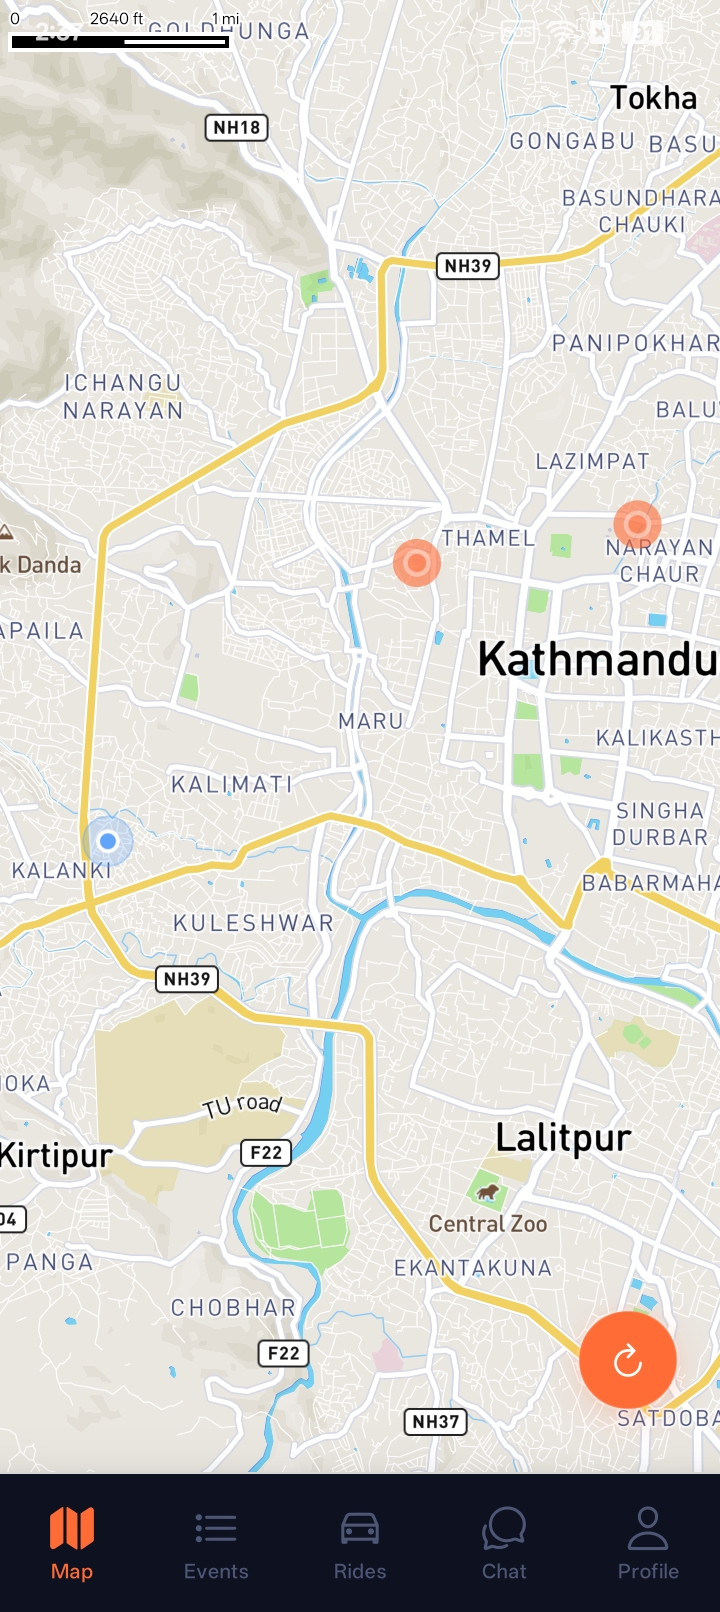
\includegraphics[width=0.5\textwidth]{blinkers.jpg}
    \caption{Figure 6.1: Real-time Geospatial Event Discovery Map Interface.}
    \label{fig:6_1}
\end{figure}

\begin{figure}[H]
    \centering
    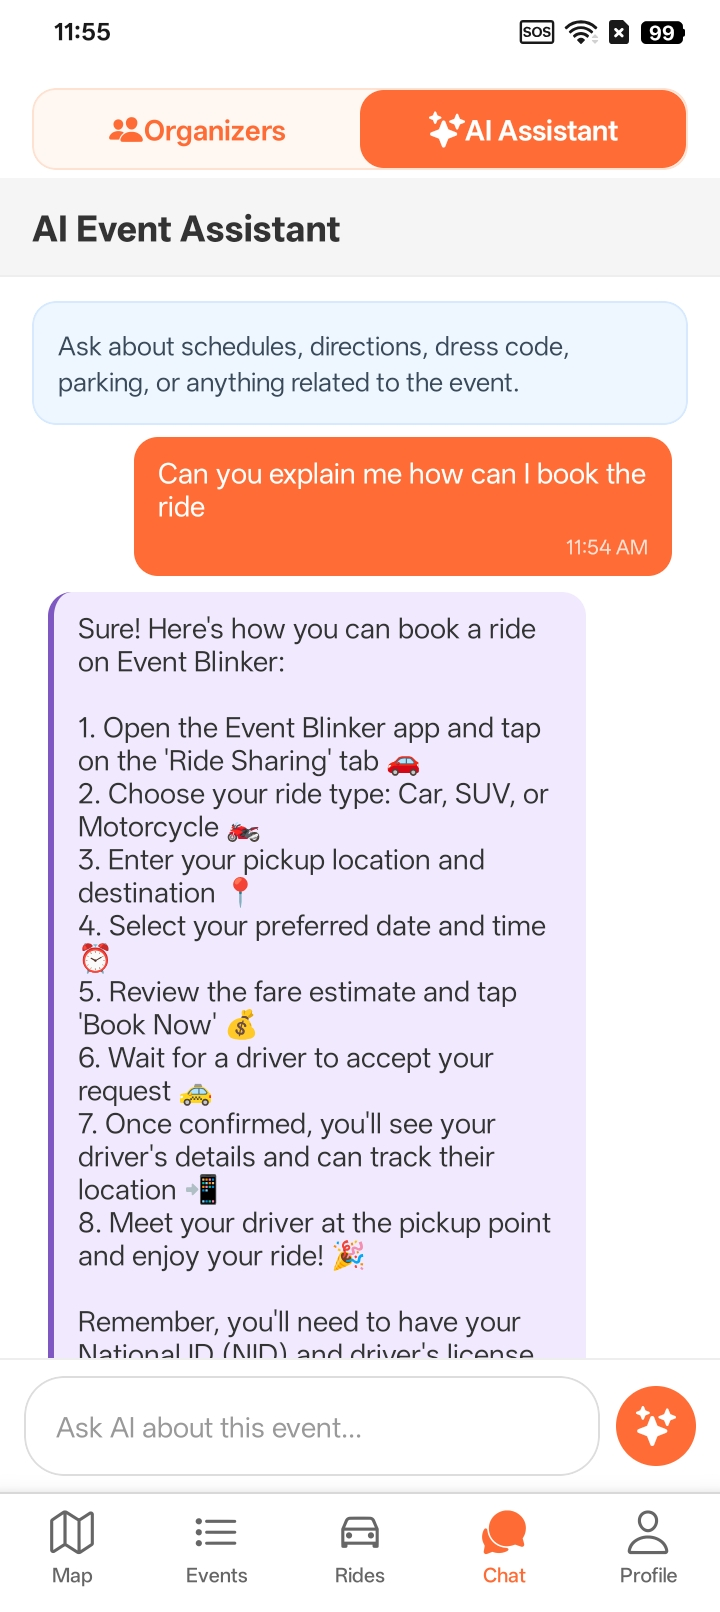
\includegraphics[width=0.5\textwidth]{aiassitant.jpg}
    \caption{Figure 6.2: Smart Assistant providing context-aware venue support.}
    \label{fig:6_2}
\end{figure}

\section{Mobility and Peer-to-Peer Workflow}
The ride-sharing infrastructure handles the transport logistics lifecycle.

\begin{figure}[H]
    \centering
    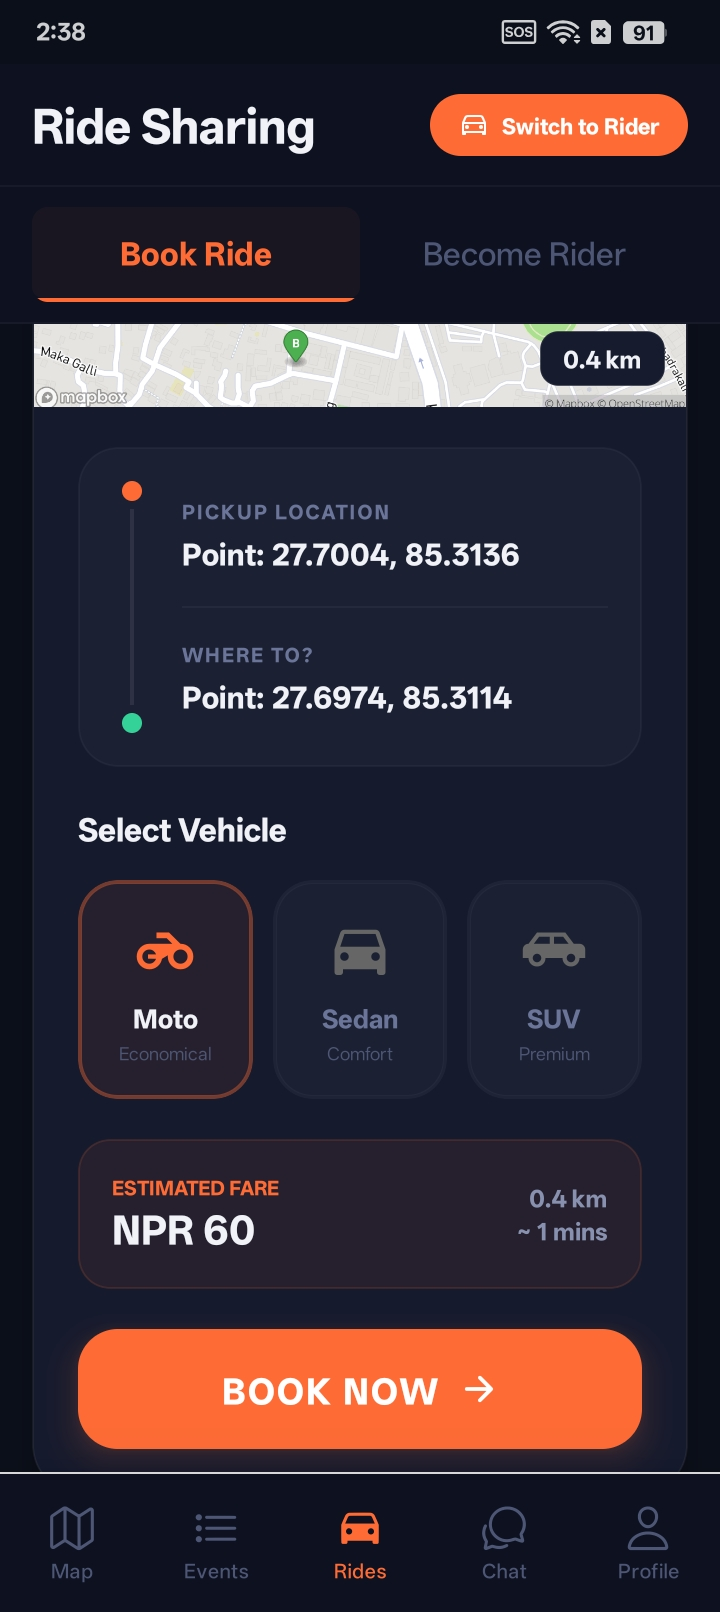
\includegraphics[width=0.5\textwidth]{ride booking.jpg}
    \caption{Figure 6.3: Peer-to-Peer Ride Booking and Fare Estimation View.}
    \label{fig:6_3}
\end{figure}

\begin{figure}[H]
    \centering
    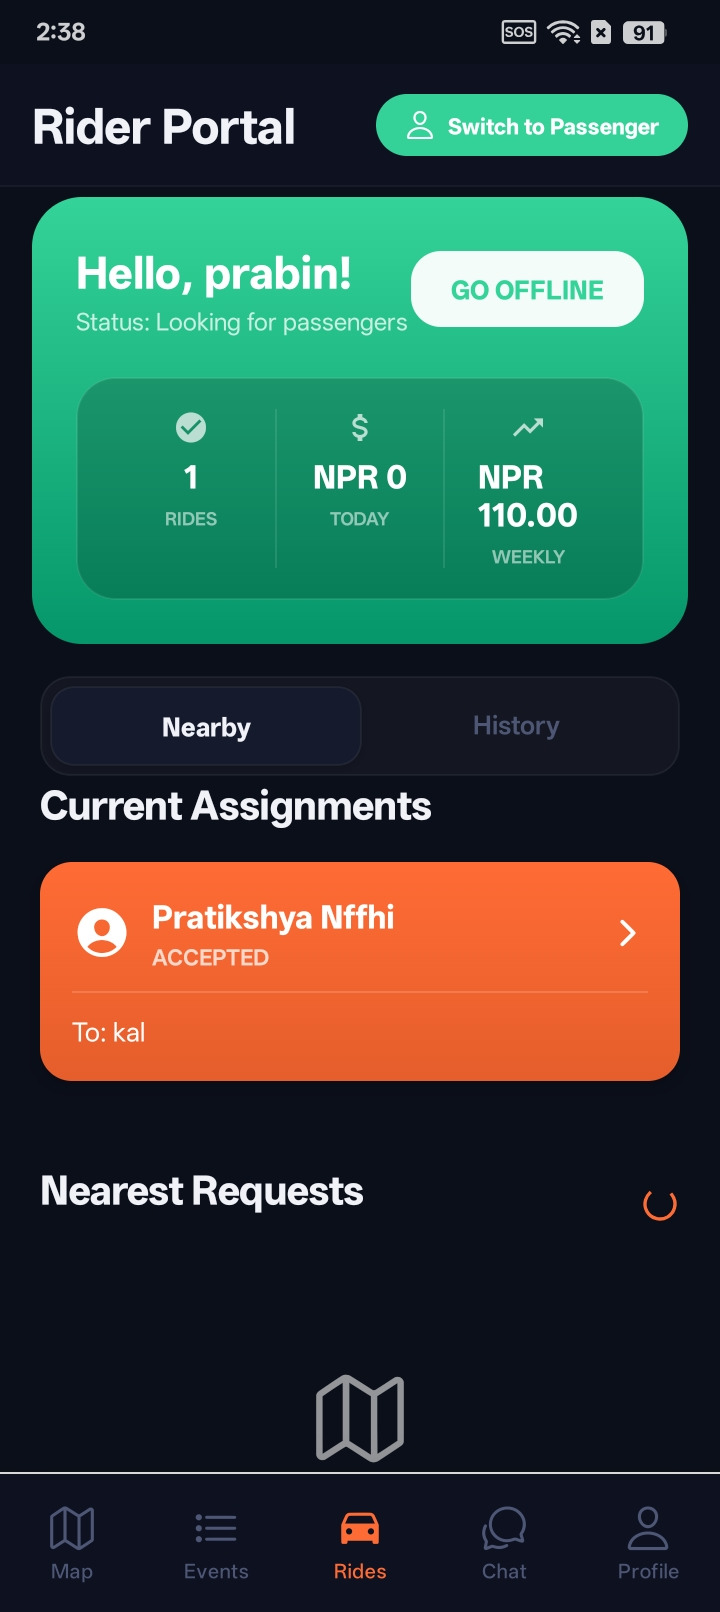
\includegraphics[width=0.85\textwidth]{rider_portal.jpg}
    \caption{Figure 6.4: Rider Profile and Document Verification Interface.}
    \label{fig:6_4}
\end{figure}

\section{Management and Administration Portals}
The system includes web infrastructures for oversight and coordination.

\begin{figure}[H]
    \centering
    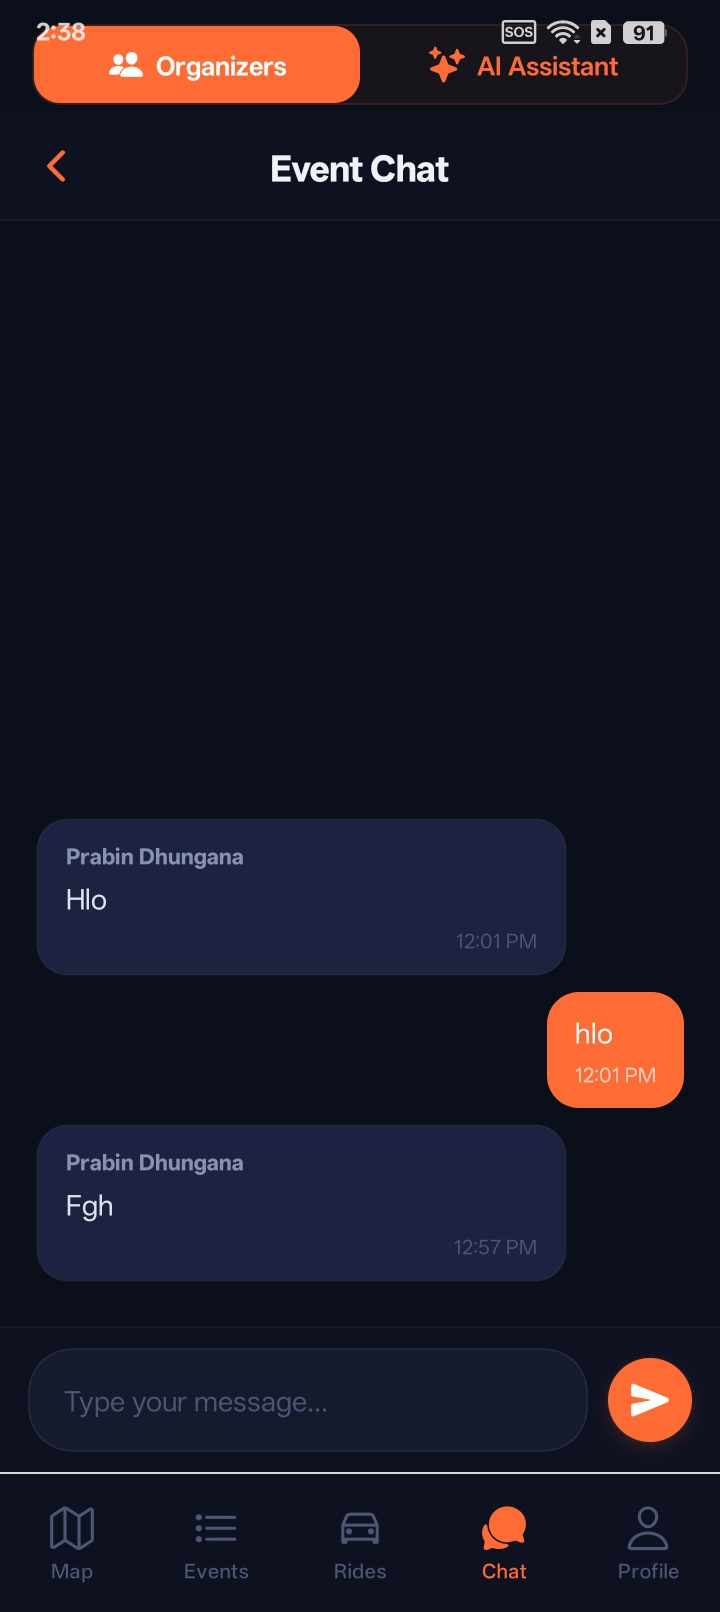
\includegraphics[width=0.85\textwidth]{eventorg_chat.jpg}
    \caption{Figure 6.5: Real-time Chat Room for Organizer-Attendee Coordination.}
    \label{fig:6_5}
\end{figure}

\begin{figure}[H]
    \centering
    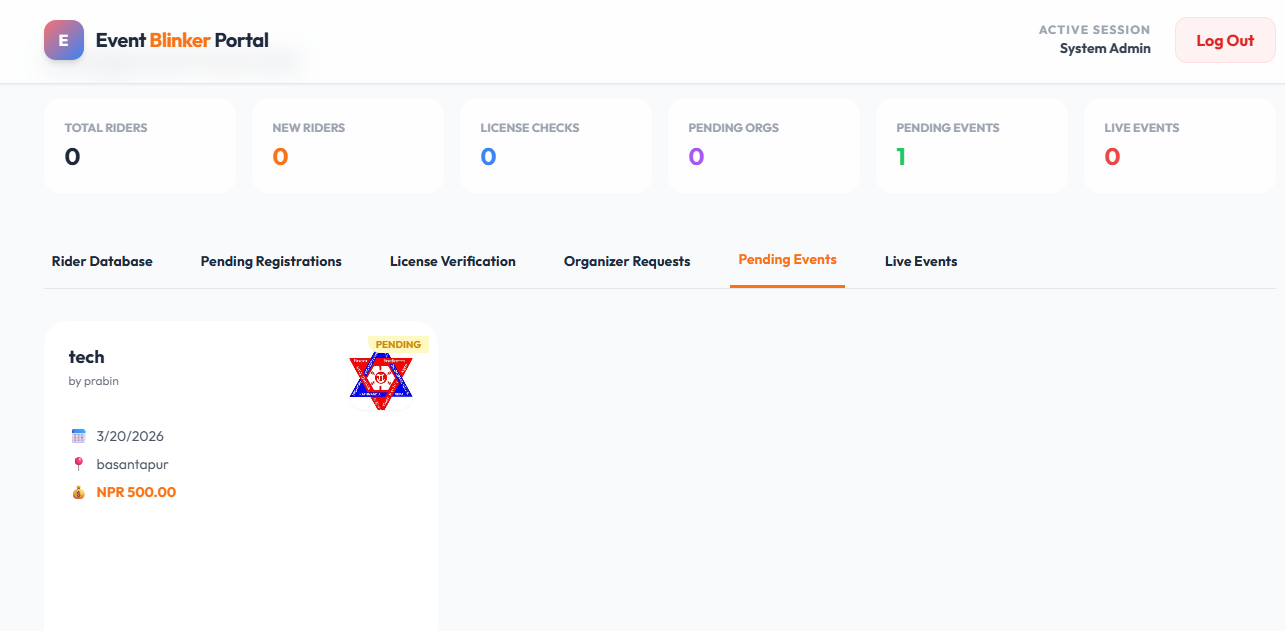
\includegraphics[width=0.85\textwidth]{organizer_portal.png}
    \caption{Figure 6.6: Organizer Dashboard displaying engagement analytics and event management.}
    \label{fig:6_6}
\end{figure}

\begin{figure}[H]
    \centering
    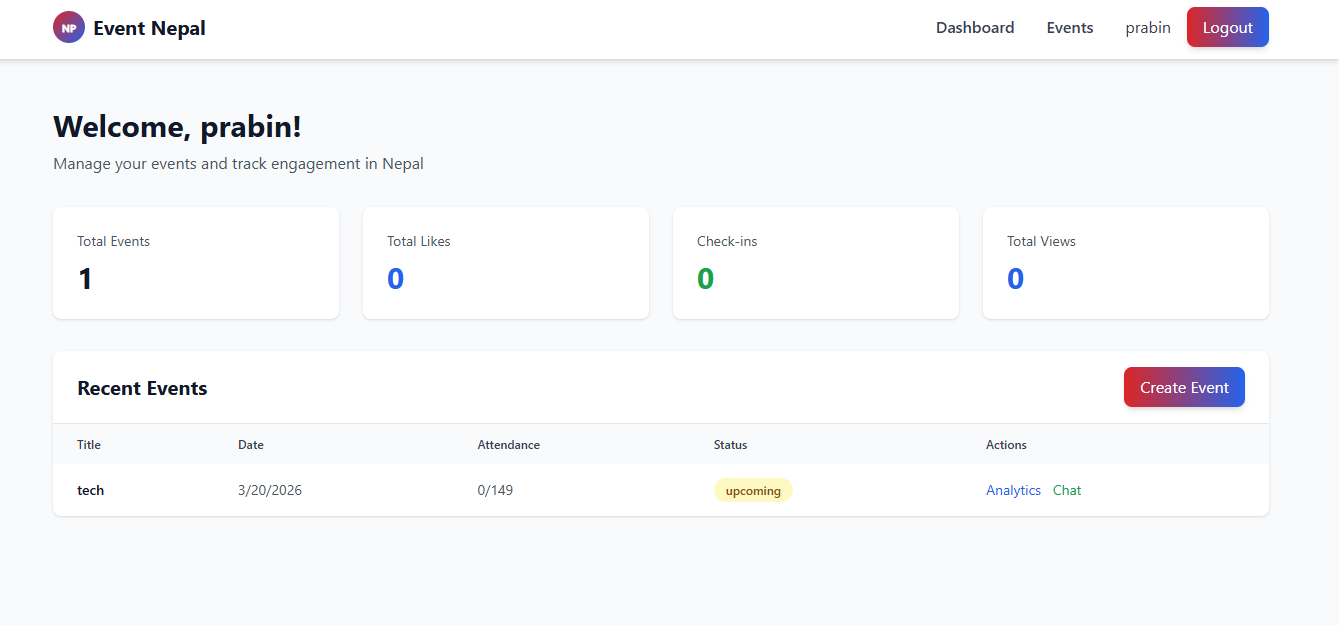
\includegraphics[width=0.85\textwidth]{admin_portal.png}
    \caption{Figure 6.7: System Administrative Portal for global user verification and moderation.}
    \label{fig:6_7}
\end{figure}

\section{Activity Monitoring and Demand Surges}
To visualize the real-time engagement of the platform, a monitoring dashboard was developed to track user activity and demand hotspots across the metropolitan area.

\begin{figure}[H]
    \centering
    
\includegraphics[width=0.85\textwidth]{activity.jpg}
    \caption{Figure 6.8: Live activity monitoring and demand surge visualization.}
    \label{fig:6_8}
\end{figure}
